\documentclass{article}
\usepackage{cmap}
\usepackage[utf8]{inputenc}
\usepackage[english,ukrainian]{babel}
\usepackage{graphicx}
\usepackage{geometry}
\usepackage{listings}
\usepackage{indentfirst}
\usepackage{subfigure}
\usepackage{caption}
\usepackage{amsmath}
\geometry{
	a4paper,
	left=20mm,
	right=20mm,
	top=20mm,
	bottom=20mm
}
\lstset{
	extendedchars=\true,
	tabsize=4,
	language=python,
	showstringspaces=false,
	showtabs=false,
	frame=lrtb,
	columns=fixed,
	keepspaces,
	breaklines=true
}
\graphicspath{ {pictures} }
\setlength{\parindent}{4em}
\newcommand\subject{Чисельні методи}
\newcommand\lecturer{доцент кафедри ПЗ\\Мельник Н.Б.}
\newcommand\teacher{асистент кафедри ПЗ\\Гарматій Г.Ю.}
\newcommand\mygroup{ПЗ-16}
\newcommand\lab{6}
\newcommand\theme{Розв'язування перевизначених систем лінійних алгебраїчних рівнянь}
\newcommand\purpose{Ознайомлення на практиці з методами розв’язування
	перевизначених систем лінійних алгебраїчних рівнянь}

\begin{document}
	\begin{large}
		\begin{titlepage}
			\thispagestyle{empty}
			\begin{center}
				\textbf{МІНІСТЕРСТВО ОСВІТИ І НАУКИ УКРАЇНИ\\
					НАЦІОНАЛЬНИЙ УНІВЕРСИТЕТ "ЛЬВІВСЬКА ПОЛІТЕХНІКА"}
			\end{center}
			\begin{flushright}
				Інститут \textbf{КНІТ}\\
				Кафедра \textbf{ПЗ}
			\end{flushright}
			\vspace{200pt}
			\begin{center}
				\textbf{ЗВІТ}\\
				\vspace{10pt}
				До лабораторної роботи № \lab\\
				\textbf{На тему}: “\textit{\theme}”\\
				\textbf{З дисципліни}: “\subject”
			\end{center}
			\vspace{90pt}
			\begin{flushright}
				
				\textbf{Лектор}:\\
				\lecturer\\
				\vspace{28pt}
				\textbf{Виконав}:\\
				
				студент групи \mygroup\\
				Коваленко Д.М.\\
				\vspace{28pt}
				\textbf{Прийняв}:\\
				
				\teacher\\
				
				\vspace{28pt}
				«\rule{1cm}{0.15mm}» \rule{1.5cm}{0.15mm} 2022 р.\\
				$\sum$ = \rule{1cm}{0.15mm}……………\\
				
			\end{flushright}
			\vspace{\fill}
			\begin{center}
				\textbf{Львів — 2022}
			\end{center}
		\end{titlepage}
		
		\begin{description}
			\item[Тема.] \theme.
			\item[Мета.] \purpose.
		\end{description}
		
		\section*{Теоретичні відомості}
		Розглянемо систему лінійних алгебраїчних рівнянь, у якій кількість
		рівнянь є більшою за кількість невідомих
		\begin{gather}
			\left\{\begin{array}{@{}l@{}}
				a_{11}x_1 + a_{12}x_2 + ... + a_{1m}x_m = b_{1},\\\nonumber
				a_{21}x_1 + a_{22}x_2 + ... + a_{2m}x_m = b_{2},\\\nonumber
				................................................\\\nonumber
				a_{n1}x_1 + a_{n2}x_2 + ... + a_{nm}x_m = b_{n}.\nonumber
			\end{array}\right.\,
		\end{gather}
		де $n>m$.
		У загальному випадку система рівнянь є несумісною. Якщо із даної системи вибрати $m$ рівнянь та розв’язати їх, то отриманий розв’язок не буде задовольняти всі рівняння системи. Тому поступимо інакше: знайдемо розв’язок системиm $x_1, x_2,...,x_m$ наближено, але щоб він задовольняв усі рівняння системи.
		
		Запишемо систему лінійних алгебраїчних рівнянь у матричному
		вигляді
		\begin{gather}\nonumber
			X=\begin{pmatrix}
				x_1\\
				x_2\\
				x_3\\
			\end{pmatrix}
			\hspace{28pt}
			A=\begin{pmatrix}
				a_{11} & a_{12} & ... & a_{1n}\\
				a_{21} & a_{22} & ... & a_{2n}\\
				... & ... & ... & ...\\
				a_{m1} & a_{m2} & ... & a_{mn}\\	
			\end{pmatrix}
			\hspace{28pt}
			B=\begin{pmatrix}
				b_1\\
				b_2\\
				...\\
				b_m
			\end{pmatrix}
		\end{gather}
		де $A$ – матриця коефіцієнтів системи розмірності n×m, X – матриця-стовпець невідомих розмірності 1×m, $B$ – матриця-стовпець вільних членів системи розмірності 1×m.
		Матричне рівняння помножимо на транспоновану матрицю $A^T$ до
		матриці $A$. У результаті отримаємо матричне рівняння
		\begin{gather}
			NX=C\nonumber
		\end{gather}
		де $N$ – матриця коефіцієнтів нормальної системи
		\begin{gather}
			N=A^TA\nonumber
		\end{gather}
		C – стовпець вільних членів
		\begin{gather}
			C=A^TB\nonumber
		\end{gather}
		Розв’язавши нормальну систему лінійних алгебраїчних рівнянь,
		отримаємо її точний розв’язок (якщо використано прямі методи) або
		наближений розв’язок (якщо використано ітераційні методи). Отриманий
		розв’язок буде наближеним для початкової системи лінійних алгебраїчних рівнянь.
		\section*{Лабораторне завдання}
		Розв’язати перевизначену систему лінійних алгебраїчних рівнянь
		методом найменших квадратів. Отриману відповідну нормальну систему
		розв’язати методом квадратного кореня.
		\begin{gather}
			\left\{\begin{array}{@{}l@{}}
				-x_1-5x_2=-6\\\nonumber
				x_1-x_2+2x_3=-3\\\nonumber
				-x_1+2x_2-5x_3=0\\\nonumber
				x_1-2x_2+3x_3=3\\\nonumber
				x_1+3x_2+2x_3=4\nonumber
			\end{array}\right.\,		
		\end{gather}
		\section*{Хід роботи}
		\begin{gather}\nonumber
			X=\begin{pmatrix}
				x_1\\
				x_2\\
				x_3\\
			\end{pmatrix}
			\hspace{28pt}
			A=\begin{pmatrix}
				-1 & -5 & 0\\
				1 & -1 & 2\\
				-1 & 2 & 5\\
				1 & -2 & 3\\
				1 & 3 & 2\\	
			\end{pmatrix}
			\hspace{28pt}
			B=\begin{pmatrix}
				-6\\
				-3\\
				0\\
				3\\
				4
			\end{pmatrix}
		\end{gather}
		\begin{gather}\nonumber
			N = \begin{pmatrix}
				5 & 3 &12\\
				3 & 43 & -12\\
				12 & 43 & -1\\
			\end{pmatrix}
			\hspace{28pt}
			C = \begin{pmatrix}
				10\\
				39\\
				42\\
			\end{pmatrix}
		\end{gather}
		\noindent\textit{\textbf{Код програми} (файл lab\_\lab.py):}
		\begin{lstlisting}
from numpy import transpose, linalg, loadtxt

def data_to_matrix(path):
	return (
		loadtxt(open(path, "rb"), delimiter=",", usecols=[0,1,2]),
		loadtxt(open(path, "rb"), delimiter=",", usecols=3),
	)

def square_root_method(A, B):
	""" Метод квадратного кореня """
	print(square_root_method.__doc__)
	L = linalg.cholesky(A)
	L_T = transpose(L)
	Y = linalg.inv(L) @ B
	print(f" L: \n {L} \n Y: \n {Y}")
	X = linalg.inv(L_T) @ Y

print("Відповідь:", [round(x, 4) for x in X])

path = input("Введіть шлях до файлу з даними: ") or "data.csv"
A, B = data_to_matrix(path)

N = transpose(A) @ A
C = transpose(A) @ B

print(f" N: \n {N} \n C: \n {C}")

square_root_method(N, C)\end{lstlisting}
		\pagebreak
		\begin{figure}[h!]
			\centering
			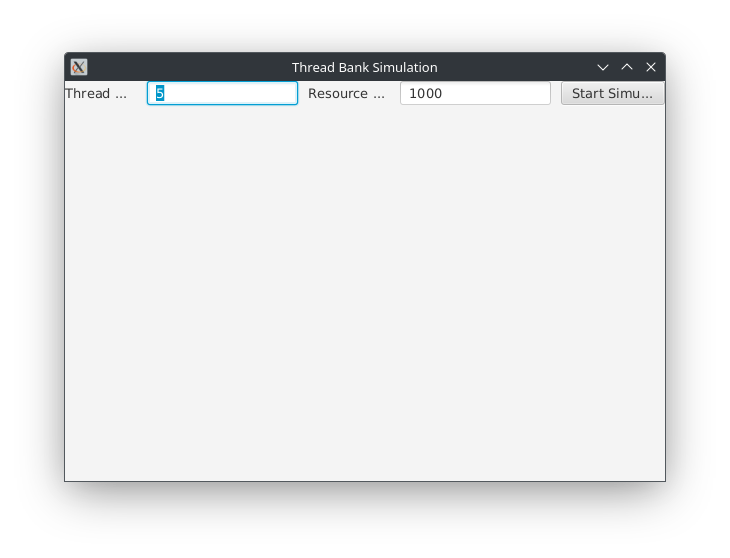
\includegraphics[scale=1]{1}
			\caption{Робота програми}
		\end{figure}
		\begin{figure}[h!]
			\centering
			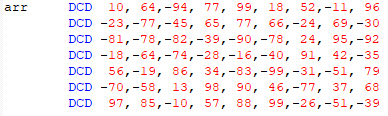
\includegraphics[scale=1]{2}
			\caption{Файл даних}
		\end{figure}
		\section*{Висновок}
		На лабораторній роботі я засвоїв практичні навички використання методу найменших квадратів та методу квадратного кореня та розробив функції для розв’язку системи лінійних алгебраїчних рівнянь.
		Наближені розв'язки системи рівнянь: $0.02; 1.06; 0.55$.
		\begin{gather}\nonumber
			\left\{\begin{array}{@{}l@{}}
				-x_1-5x_2=-6\\\nonumber
				x_1-x_2+2x_3=-3\\\nonumber
				-x_1+2x_2-5x_3=0\\\nonumber
				x_1-2x_2+3x_3=3\\\nonumber
				x_1+3x_2+2x_3=4\nonumber
			\end{array}\right.\,
			\hspace{28pt}
			\left\{\begin{array}{@{}l@{}}
				-5.28=-6,\\\nonumber
				0.06=-3,\\\nonumber
				-4.89=0,\\\nonumber
				-0.45=3,\\\nonumber
				4.3=4,\nonumber
			\end{array}\right.\,
			\hspace{28pt}
			\left\{\begin{array}{@{}l@{}}
				\varepsilon_1=0.72\\\nonumber
				\varepsilon_2=3.06\\\nonumber
				\varepsilon_3=4.89\\\nonumber
				\varepsilon_4=3.45\\\nonumber
				\varepsilon_5=0.3\nonumber
			\end{array}\right.\,			
		\end{gather} 
	\end{large}
\end{document}
